\section{Anpassung in der Docker Containerisierung}\label{subsec:docker-containerisierung}

Bereits im Praxismodul I wurde mit Docker Containern für die lokale Entwicklung gearbeitet.
Dieses Semester kamen zwei Aspekte hinzu, die auf dem angeeigneten Wissensstand aus dem vorherigen Semester aufgebaut haben - Multiplattform Images und das Deployen von Docker Anwendungen auf einem Server, der über das öffentliche Netz erreichbar ist.

\subsection{Multiplattform Images}\label{subsubsec:multiplattform-images}
Während der Durchführung des Projekts ist ein Teammitglied auf einen ARM-Prozessor umgestiegen.
Letztes Semester erfolgte die Programmierung ausschließlich auf x86 Windows Maschinen, wodurch Docker Images, die auf einer Maschine gebaut wurden, problemlos auf allen anderen Maschinen funktioniert haben.
Images, die für x86 Architektur gebaut wurden, funktionieren nicht auf ARM-Maschinen.
Eine Lösung wurde hier in Multiplattform Docker Images gefunden.
Wird ein solches Image aus einer Registry auf den eigenen Rechner gezogen, so erkennt Docker automatisch die Architektur, die benötigt wird.
So lässt sich bspw eine x86 und eine ARM Version des gleichen Docker Images in Docker Hub unter dem gleichen Registry Eintrag hosten.
Beim pullen des Images wird dann automatisch erkannt, für welche Architektur das Image benötigt wird.
In Dockerhub sieht ein Multiplattform Image dann wie folgt aus:

\begin{figure}[h]
  \centering
  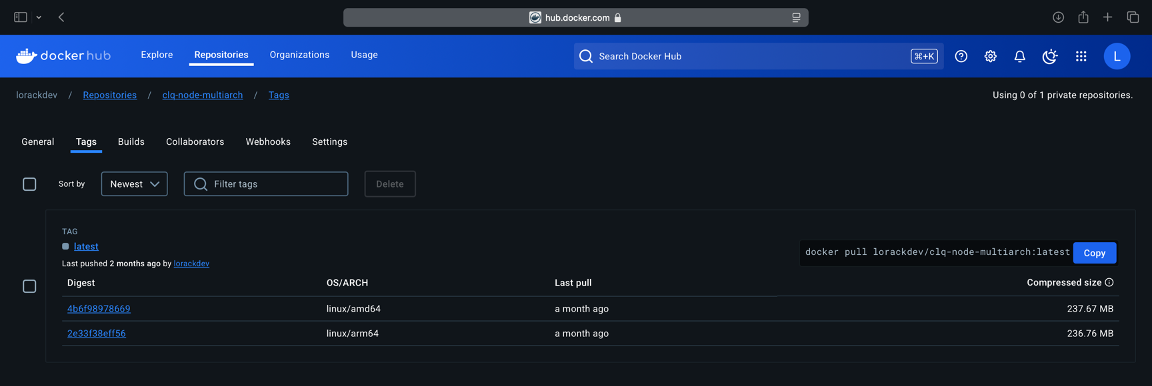
\includegraphics[width=0.7\textwidth]{docker_hub}
  \caption{Multiplattform Images in Docker Hub}
  \label{fig:docker_hub}
\end{figure}

Bevor die Images gehostet werden können, müssen diese aber zuerst gebaut werden.
Das Bauen von Multiplattform Images erfolgt mit einer Komponente von Docker, die sich buildx nennt.
Buildx selbst ist hierbei eine Anwendung, die selbst in einem Docker Container läuft.
Damit interagiert wird über den üblichen docker build befehl, welcher nun aber um den buildx Befehl erweitert wird.
Das buildx Packet wird bei den aktuellsten Docker Versionen mitgeliefert, so muss der Container einfach wie folgt gestartet werden:

\vspace{1em}
\begin{lstlisting}[label={lst:lst-shell-buildx-setup}]
docker buildx create --name multi-arch-build --use
\end{lstlisting}
\vspace{1em}

Da verschiedene Images gebaut werden müssen, wurde folgendes Shell-Script entworfen, um den manuellen Aufwand zu verringern.
Übergeben werden hier der Name, den das Image tragen soll sowie die Dockerfile, die als Basis für das Image dienen soll.

\vspace{1em}
\begin{lstlisting}[label={lst:lst-shell-buildx-build}]
#!/bin/bash

# Check if IMAGE_NAME is passed
if [ -z "$1" ]; then
  echo "Error: IMAGE_NAME is not provided."
  echo "Usage: $0 <image_name> <dockerfile_path>"
  exit 1
fi

# Check if DOCKERFILE_PATH is passed
if [ -z "$2" ]; then
  echo "Error: DOCKERFILE_PATH is not provided."
  echo "Usage: $0 <image_name> <dockerfile_path>"
  exit 1
fi

# Check if FULL_IMAGE_NAME is passed
if [ -z "$2" ]; then
  echo "Error: FULL_IMAGE_NAME is not provided."
  echo "Usage: $0 <image_name> <dockerfile_path>"
  exit 1
fi

IMAGE_NAME="$1"
DOCKERFILE_PATH="$2"
FULL_IMAGE_NAME="$3"

# Ensure you are logged in to the Docker registry
docker login || { echo "Docker login failed"; exit 1; }

# Build and push the Docker image
docker buildx build --platform linux/amd64,linux/arm64 -t ${FULL_IMAGE_NAME} -f ${DOCKERFILE_PATH} --push .
\end{lstlisting}
\vspace{1em}

Die Push Flag am Ende des Befehls lädt gleichzeitig das neue Image in die Container Registry, in die der User eingelogt ist, hoch.
Im Fall dieses Projekts werden alle Images in Docker Hub gehostet.

\subsection{Deployment auf vServer}\label{subsec:deployment-auf-vserver}
Das Hosten der Docker Images in Docker Hub hat das Deployen auf dem vServer sehr einfach gestaltet.
Bei dem Server handelt es sich um eine ARM-Maschine, spätestens hier wären Multiplattform Images benötigt gewesen.
Zuerst wurde der SSH Key des Servers als Deploy Key auf GitHub hinterlegt.
Deploy Keys können pro Projekt hinterlegt werden und auf Read-Only geschaltet werden.
Sollten sich Angreifer einen Zugriff auf den Server verschaffen können, ist das Repository des Projekts somit vor ungewolltem Löschen und Überschreiben geschützt.
Mit anderen Repositories, die an den Account gebunden sind, kann nicht interagiert werden.
Das Repository wurde auf den Server geklont, da dieses die docker-compose.yaml Datei beinhaltet.
Um den Docker Compose Befehl ausführen zu können, muss jedoch eine Lese Berechtigung für die Docker Images im Docker Hub bestehen.
Hierzu wurde auf Docker Hub ein Token erstellt, mit Read-Only Berechtigungen, welchen zum Authentifizieren mit Docker Hub genutzt wurde.
Somit lassen sich die Images nun auf den Server pullen.

Im Zuge der Konfiguration des Reverse Proxies wurde ein separater branch im Git Repository erstellt.
Aktuell wird dieser Weg noch so gewählt, da die Konfiguration der neuen Container rein für den Server gedacht ist.
Wie in Abschnitt \ref{subsubsec:reverse-proxy} beschrieben, kamen drei neue Container hinzu, die in der docker-compose.yaml Datei hinzugefügt wurden.
Dies umfasst die Container für den Nginx Reverse Proxy, Certbot (Zertifikate) und einen Test-Webserver.
Die Docker Compose Datei sieht nun wie folgt aus:
\vspace{1em}
\begin{lstlisting}[label={lst:lst-docker-compose-yaml}]
# version: '3'
services:
  web:
    container_name: collectiqo-web-1
    image: clq-app
    env_file: ./.env.docker
    ports:
      - "${PORT}:${PORT}"
    volumes:
      #- ~/.certificates/collectiqo/:/root/.certificates/collectiqo:ro # mount local keys into container for dev purposes
      - /home/collectiqo/local_cert/collectiqo_rs:/root/.certificates/collectiqo:ro # mount local keys into container for dev purposes
    networks:
      - proxy-network
      #- app-network
  mysql:
    container_name: collectiqo-mysql-1
    image: lorackdev/clq-mysql-multiarch
    restart: always
    environment:
      MYSQL_ROOT_PASSWORD: ${MYSQL_DATABASE_PASSWORD}
    ports:
      - "${MYSQL_DATABASE_PORT}:${MYSQL_DATABASE_PORT}"
    networks:
      - proxy-network
      #- app-network
  mongodb:
    container_name: collectiqo-mongodb-1
    image: mongo:latest
    restart: always
    ports:
      - "${MONGO_DATABASE_PORT}:${MONGO_DATABASE_PORT}"
    environment:
      MONGO_INITDB_ROOT_USERNAME: ${MONGO_DATABASE_USER}
      MONGO_INITDB_ROOT_PASSWORD: ${MONGO_DATABASE_PASSWORD}
    networks:
      - proxy-network
      #- app-network
  test-webserver:
    container_name: test-webserver
    image: arm64v8/httpd:latest
    restart: unless-stopped
    volumes:
      - ./webtest:/usr/local/apache2/htdocs:ro
    networks:
      - proxy-network
  nginx-reverse-proxy:
    container_name: nginx-reverse-proxy
    image: nginx:latest
    restart: unless-stopped
    ports:
      - "80:80"
      - "443:443"
    volumes:
      - ./nginx/nginx.conf:/etc/nginx/nginx.conf:ro
      - ./certbot/conf:/etc/letsencrypt/:ro
      - ./certbot/www:/var/www/certbot/:ro
    networks:
      - proxy-network
  certbot:
    container_name: certbot
    image: certbot/certbot:latest
    volumes:
      - ./certbot/conf:/etc/letsencrypt/:rw
      - ./certbot/www:/var/www/certbot/:rw
    networks:
      - proxy-network
    depends_on:
      - nginx-reverse-proxy
networks:
  app-network:
    driver: bridge
  proxy-network:
    driver: bridge
\end{lstlisting}
\vspace{1em}

Diese verändert sich zur vorherigen Version insofern, dass sie nun auf Umgebungsvariablen für Werte wie Ports und Passwörter angewiesen ist.
Auch dem Container des NodeJS Servers wird eine .env Datei übergeben.
Da die .env Datei sensible, projektspezifische Daten beinhaltet, liegt im Repository nur eine Beispieldatei (.env.example), die nur den Key ohne die dazugehörige Value angibt.
Diese Datei wurde auf dem Server dann mit entsprechenden Values für die einzelnen Keys befüllt.
Schlussendlich wurde die docker-compose.yaml mit einem einfachen docker compose up ausgeführt, wodurch die Apps nun auf dem Server laufen.

Im nächsten Schritt soll das Deployment neuer Versionen der App automatisiert werden, da das Ausrollen einer neuen Version immer das manuelle Ausführen der Docker Compose beinhaltet und ggf. das aktualisieren des Git Repositories.
Die Netzwerkkonfiguration der Container ist ebenfalls noch nicht optimal, zwei Netzwerke sind angedacht um u.a. die Datenbanken gezielter zu schützen.
Das Portmapping der Container ist ebenfalls noch nicht optimal, da die Ports der NodeJS App und der Datenbanken bei einem externen Portscan aktuell sichtbar sind.
Zusätzlich kommt es gelegentlich zu Problemen da die Datenbanken nicht schnell genug starten und der NodeJS Server somit nicht auf die Datenbanken zugreifen kann.
Es bedarf also noch einiger Optimierungen, um die Containerisierung der Anwendungen zu perfektionieren.